% **********************************************************
%				 	  ELEMENTOS TEXTUAIS				   *
% **********************************************************



% Deixar três (3) linhas em branco antes dos títulos de cápitulos
% %%%%%%%%%%%%%%%%%%%%%%%%%%%%%%%%%%%%%%%%%%%%%%%%%%%%%%%%%%%%%%%%%%%%%%%%%
\chapter[Introdução]{Introdução} \label{ch:introducao}
% %%%%%%%%%%%%%%%%%%%%%%%%%%%%%%%%%%%%%%%%%%%%%%%%%%%%%%%%%%%%%%%%%%%%%%%%%
% Deixar uma (1) linha em branco após cada título

A introdução deve contextualizar o tema do trabalho, apresentar a motivação para a pesquisa e descrever o problema a ser investigado. A introdução também deve incluir as seguintes seções: Justificativa, Objetivo, Objetivo Geral, Objetivos Específicos e Metodologia.



% Deixar três (2) linhas em branco antes dos títulos das seções
% -------------------------------------------------------------------------
\section{Justificativa} \label{sec:justificativa}
% -------------------------------------------------------------------------
% Deixar uma (1) linha em branco após o título da seção, para separar do texto
Explicação sobre a relevância do estudo, destacando sua importância acadêmica, científica ou prática.


% -------------------------------------------------------------------------
\section{Objetivo} \label{sec:objetivo}
% -------------------------------------------------------------------------

Definição clara do que o trabalho pretende alcançar.


% -------------------------------------------------------------------------
\subsection{Objetivo Geral} \label{sec:objetivo-geral}
% -------------------------------------------------------------------------

Descrição do propósito central do estudo.


% -------------------------------------------------------------------------
\subsection{Objetivos Específicos} \label{sec:objetivos-especificos}
% -------------------------------------------------------------------------
Lista de metas detalhadas que, quando atingidas, contribuem para o objetivo geral.
Exemplo:
\begin{alineas} % {enumerate} -> para números, {alineas} -> para letras
    \item Analisar e inferir ...
    
    \item Modelar e implementar uma ...
    
    \item Realizar análise e implementação do ...
    
    \item Desenvolvimento de um ...
\end{alineas}


% -------------------------------------------------------------------------
\section{Metodologia} \label{sec:metodologia}
% -------------------------------------------------------------------------
Descrição dos métodos utilizados para realizar o estudo, incluindo tipo de pesquisa, técnicas de coleta de dados, ferramentas e procedimentos adotados.
	

% %%%%%%%%%%%%%%%%%%%%%%%%%%%%%%%%%%%%%%%%%%%%%%%%%%%%%%%%%%%%%%%%%%%%%%%%%
\chapter{Referencial Teórico} \label{ch:referencia-teorico}
% %%%%%%%%%%%%%%%%%%%%%%%%%%%%%%%%%%%%%%%%%%%%%%%%%%%%%%%%%%%%%%%%%%%%%%%%%

Este é um parágrafo introdutório que tem por objetivo introduzir o que será apresentado neste capítulo.

Neste capítulo deve ser apresentado uma revisão da literatura sobre o tema do trabalho, apresentando conceitos, teorias e estudos relevantes que fundamentam a pesquisa. Pode ser subdividido conforme necessário. 

Exemplo 1 de citação, \cite{almeida2022}\\
Exemplo 2 de citação, \citeonline{almeida2022}\\ 
% Deixar duas (2) linhas em branco antes do o título de uma seção
Lista com citações de  diferentes tipos de documentos, para gerar o exemplo de\\ \textbf{Referências} ao final do documento.\\ \\
Dissertação, \cite{almeida2022}\\
Trabalho publicado em Conferência, \cite{cbsoft2023}\\
Página web, \cite{ferreira2020}\\
Manual, \cite{latex2023}\\
Capitulo de livro, \cite{mendes2019}\\
Relatório técnico, \cite{oliveira2020}\\
Livro, \cite{linden2012}\\
Tese de doutorado, \cite{rodrigues2021}\\
Artigo científico, \cite{silva2023}\\
Livro de Conferência, \cite{souza2022}


% -------------------------------------------------------------------------
\section{Título da Seção} \label{sec:definir-tituto-da-secao}
% -------------------------------------------------------------------------
% Deixar uma (1) linha em branco após o título da seção, para separar do texto
Discussão detalhada de um dos tópicos fundamentais para o entendimento do problema abordado. \\ Caso necessário, pode ser criado subseções


% -------------------------------------------------------------------------
\section{Título da Subseção} \label{sec:definir-outro-tituto-de-secao}
% -------------------------------------------------------------------------
Discussão detalhada parte de um dos tópicos fundamentais para o entendimento do problema abordado.
\begin{figure} [htb]
    \begin{center}
	 \caption{\label{fig:ag}Esquema de um algoritmo genético}
        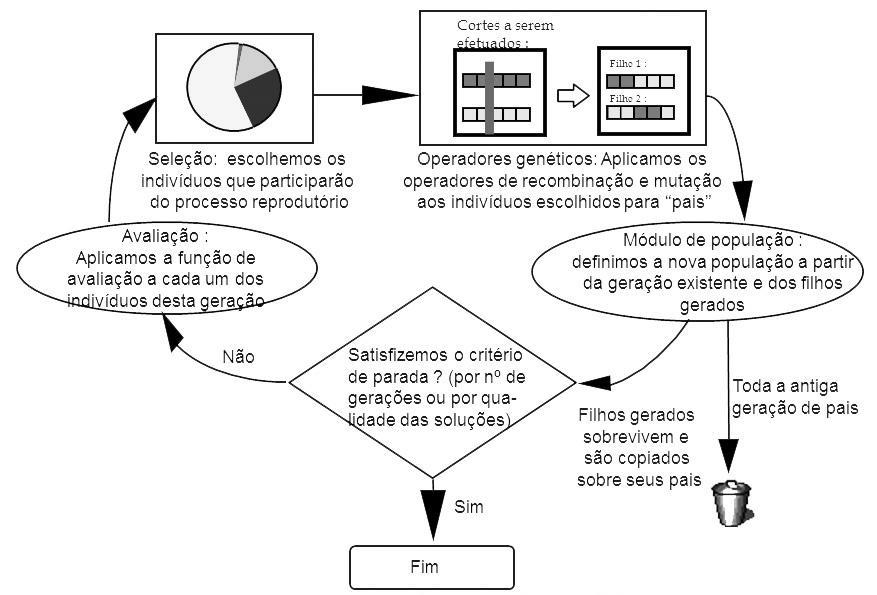
\includegraphics[scale=0.6]{imagens/nome-cap/nome-sec/esquemaAlgGenetico_pag64.png}
	\legend{Fonte: \citeonline[p. 64]{linden2012}.}
    	\end{center}
    \end{figure}
    
Incluindo uma figura de autoria própria.
\begin{figure} [htb]
\begin{center}
	 \caption{\label{fig:ambiente}Ambiente abordado}
	    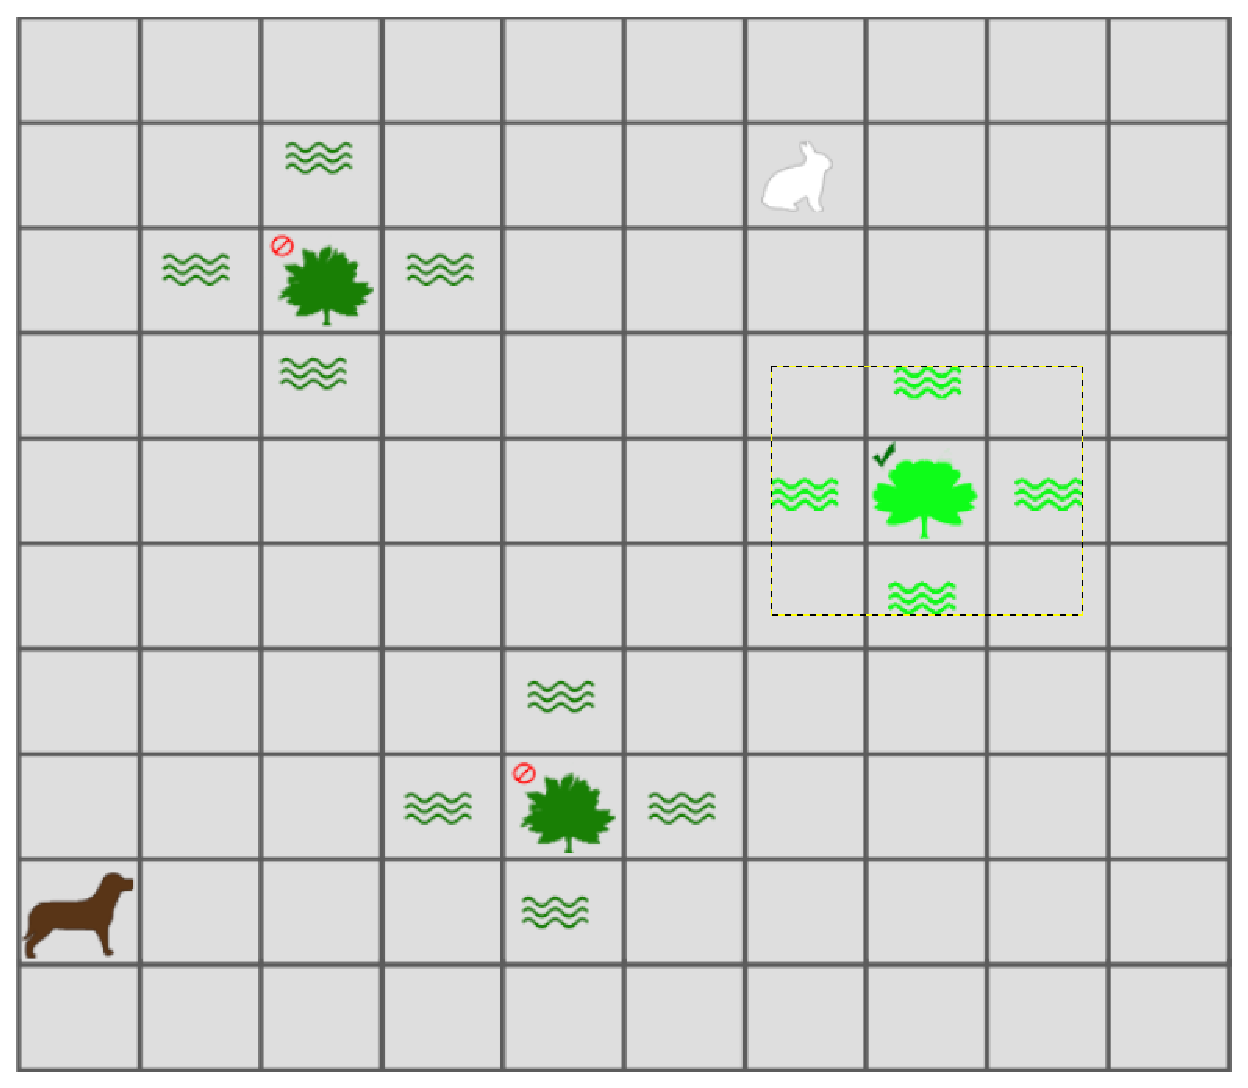
\includegraphics[scale=0.3]{imagens/nome-cap/nome-sec/ambiente.eps}
	\legend{Fonte: autoria própria.}
    \end{center}
\end{figure}


% %%%%%%%%%%%%%%%%%%%%%%%%%%%%%%%%%%%%%%%%%%%%%%%%%%%%%%%%%%%%%%%%%%%%%%%%%
\chapter{Desenvolvimento} \label{ch:definir-um-label-titulo-de-capitulo}
% %%%%%%%%%%%%%%%%%%%%%%%%%%%%%%%%%%%%%%%%%%%%%%%%%%%%%%%%%%%%%%%%%%%%%%%%%
A parte referente ao ``Desenvolvimento'' pode ser dividido em dois ou mais capítulos, e cada capítulo pode ser dividido em seções e subseções caso seja necessário para melhorar a apresentação e a legibilidade do documento.

Para referenciar a tabela você pode usar o comando "autoref" ex: \autoref{tab:resultados1}, ou o "ref", ex: \ref{tab:resultados1}

\begin{table}[htb]
\centering
\caption{Exemplo de tabela conforme a ABNT}
\label{tab:resultados1}
\begin{tabular}{p{0.3\textwidth} p{0.3\textwidth} p{0.3\textwidth}} % Ajuste das larguras das colunas
    \hline
    \textbf{Coluna 1} & \textbf{Coluna 2} & \textbf{Coluna 3} \\
    \hline
    Informação 1 & Informação 2 & Informação 3 \\
    Informação 4 & Informação 5 & Informação 6 \\
    Informação 7 & Informação 8 & Informação 9 \\  
    \hline
\end{tabular}
\legend{Fonte: autoria própria.}
\end{table}

\begin{table}[htb]
\centering
\caption{Exemplo de tabela conforme a ABNT}
\label{tab:resultados2}
\begin{tabular}{>{\centering\arraybackslash}p{0.3\textwidth}  >{\centering\arraybackslash}p{0.3\textwidth}  >{\centering\arraybackslash}p{0.3\textwidth}} % Ajuste das larguras das colunas
    \hline
    \textbf{Coluna 1} & \textbf{Coluna 2} & \textbf{Coluna 3} \\
    \hline
    Informação 1 & Informação 2 & Informação 3 \\
    Informação 4 & Informação 5 & Informação 6 \\
    Informação 7 & Informação 8 & Informação 9 \\  
    \hline
\end{tabular}
\legend{Fonte: autoria própria.}
\end{table}




\begin{table}[h]
    \centering
    \caption{Exemplo de tabela conforme a ABNT}
    \label{quad:exemplo}
    \begin{tabular}{p{3cm} p{4cm} p{3cm}}
        \hline%\toprule
        \textbf{Coluna 1} & \textbf{Coluna 2} & \textbf{Coluna 3} \\
        \hline%\midrule
        Informação 1 & Informação 2 & Informação 3 \\
        Informação 4 & Informação 5 & Informação 6 \\
        Informação 7 & Informação 8 & Informação 9 \\
        \hline%\bottomrule
    \end{tabular}
    \legend{Fonte: \citeonline{linden2012}.}
\end{table}

% %%%%%%%%%%%%%%%%%%%%%%%%%%%%%%%%%%%%%%%%%%%%%%%%%%%%%%%%%%%%%%%%%%%%%%%%%
\chapter{Conclusão} \label{ch:conclusao}
% %%%%%%%%%%%%%%%%%%%%%%%%%%%%%%%%%%%%%%%%%%%%%%%%%%%%%%%%%%%%%%%%%%%%%%%%%

A conclusão deve apresentar um resumo das principais descobertas do trabalho, avaliação do cumprimento do objetivos propostos na seção \textbf{objetivos} e possíveis sugestões para trabalhos futuros.